\documentclass[border=10pt]{standalone}
\usepackage{tikz}\usepackage{amsmath}\usetikzlibrary{arrows.meta}
\begin{document}
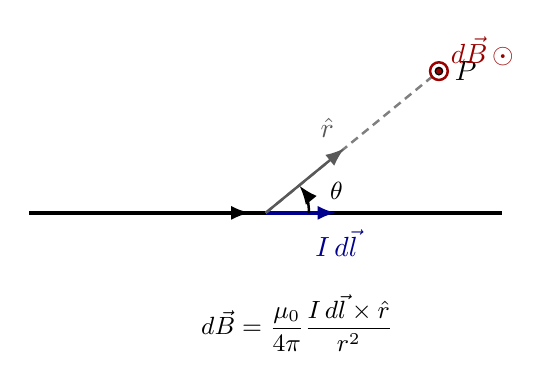
\begin{tikzpicture}[line width=0.9pt,>={Latex[length=2.4mm]}]
  \draw[line width=1.3pt] (-3,0)--(3,0);
  \draw[->,line width=1.1pt] (-1.2,0)--(-0.2,0);
  \draw[->,blue!55!black,line width=1.4pt] (0,0)--(0.9,0) node[below=2pt]{$I\,d\vec l$};
  \coordinate (P) at (2.2,1.8);
  \fill (P) circle(1.6pt) node[right=2pt]{$P$};
  \draw[densely dashed,gray] (0,0)--(P);
  \draw[->,gray!70!black] (0,0)--(1.0,0.82) node[above left]{$\hat r$};
  \draw[->] (0.55,0) arc (0:39:0.55); \node at (0.9,0.28){\small$\theta$};
  \draw[red!60!black] (P) circle(3.2pt); \fill[red!60!black] (P) circle(1pt);
  \node[red!60!black] at (2.75,2.05){$d\vec B\,\odot$};
  \node at (0.4,-1.4){\small $\displaystyle d\vec B=\frac{\mu_0}{4\pi}\frac{I\,d\vec l\times\hat r}{r^2}$};
\end{tikzpicture}
\end{document}
